\section{Hauptteil}
\label{sec:hauptteil}

\subsection{Auswirkungen des Semantischen Webs auf die Gesellschaft}

Schon heute drehen sich die meisten der regelmäßig ausgeführtem Aktivitäten im Internet um \buzz{Informationen} oder gar \buzz{Wissen}, nicht um \buzz{Daten}. So sind 56\% der im Digitalindex 2014 befragten Deutschen überzeugt, im Internet die automatisch die aktuellsten Informationen zu finden, 60\% sucht benötigte Informationen zuerst im Netz\footnote{vgl. \cite{d21}, Seite 6}. Die Erwartungen bzgl. Aktualität und Informationsgehalt an das \ac{WWW} sind also sehr hoch. 

\begin{figure}[H]
\begin{center}
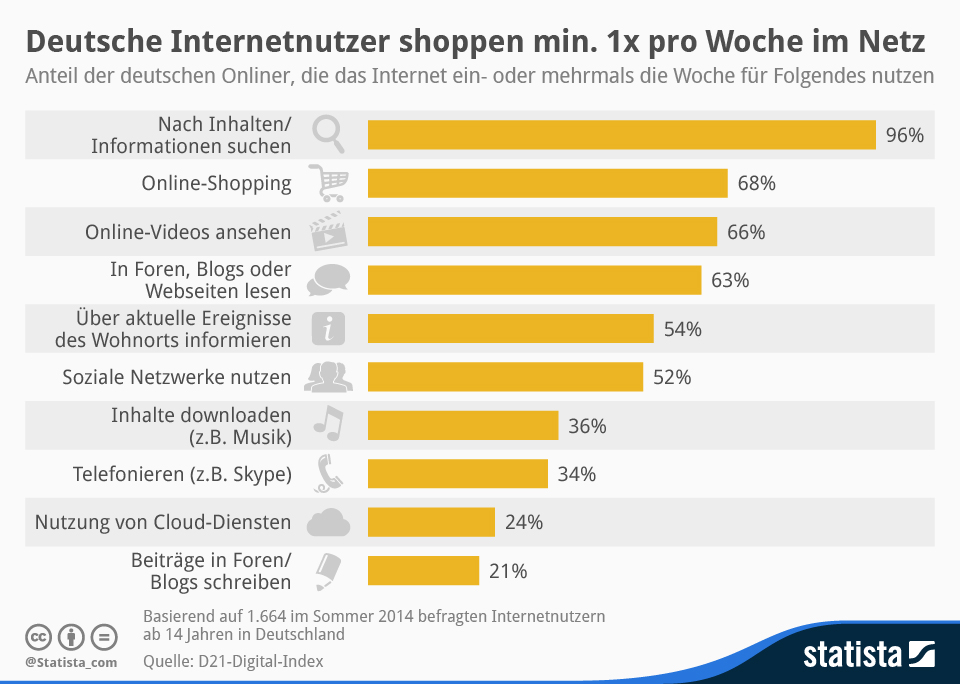
\includegraphics[width=0.67\textwidth]{inetnutzung.jpg}
\caption[Internetnutzung in Deutschland 2014]{Internetnutzung in Deutschland 2014\protect\footnotemark}
\label{pic:inetnutzung}
\end{center}
\end{figure}
\footnotetext{\cite{d21}, Seite 37}

Unter den Top 10 der regelmäßig durchgeführten Tätigkeiten der Befragten im Web finden sich die informationsorientierten Tätigkeiten „nach Inhalten/Informationen suchen“ auf Platz eins, „über aktuelle Ereignisse des Wohnorts informieren“ auf Platz 6 und die Erfassung eigener Daten auf Platz 10\footnote{vgl. \cite{d21}, Seite 37}. Weitere Tätigkeiten wie „Soziale Netzwerke nutzen“ (Platz 7) bzw. „Online--Videos ansehen“ (Platz 3) sowie „Online--Shopping“ (Platz 2) nutzen Internetangebote, die per Design sehr gut mit Taxonomien, Meta--Daten und Verknüpfungen ausgestattet sind.

In den TV--Werbespots von Google und Apple werden Verbraucher gezielt auf entsprechend Formulierte Anfragemöglichkeiten hingewiesen\footnote{z.B. „Ok Google, wie lange brauche ich nach Spandau?“}. Somit werden die Möglichkeiten wie Routenplanung, Musiktitelerkennung, Wettervorhersage und andere, die schon heute durch einzelne Anwendungen zur Verfügung gestellt werden in einer Oberfläche Gebündelt und in das Bewusstsein der Verbraucher gebracht.

\label{probleme}
Neben dem offensichtlichen Nutzen des \ac{WWW} bringt die Entwicklung des Webs auch negative Auswirkungen auf die Gesellschaft. 
Dies äußert sich mit der Besorgnis von 60\% der Nutzer über die im Internet möglicherweise verfügbaren persönlichen Daten\footnote{vgl. \cite{d21}, Seite 6}. Bei der Nutzung von Webdiensten der öffentlichen Verwaltung haben 65\% der Befragten Angst vor Datendiebstahl, und 73\% der Deutschen haben ein starkes Interesse daran, wie Behörden mit den Daten der Bürger umgeht\footnote{vgl. \cite{d21gov}, Seite 9 bzw. Seite 34}.  Sowohl fiktive\footnote{vgl. \cite{orwell}} also auch reale\footnote{vgl. \cite{wp:stasi}} Unrechtsstaaten basieren auf der intensiven Erfassung und Auswertung von personenbezogener Daten der Bürger, was entsprechende Befürchtungen nährt und erklärt.

Man kann davon ausgehen, dass mit weiter wachsenden Datenmengen, aber auch durch entsprechenden Wachstum an generierten und erfassten Informationen und Wissen sowohl die positiven Erwartungen als auch die Befürchtungen und Ängste in der Bevölkerung zunehmen werden.

\subsection{Auswirkungen des Semantischen Webs auf die Wirtschaft}

Schon heute haben Unternehmen erkannt, dass es nicht ausreicht, immer mehr Daten anzuhäufen. Der Schritt von \buzz{Big Data} zu \buzz{Big Information} bringt Benutzerfreundlichkeit und echten Mehrwert für Unternehmen\footnote{vgl. \cite{odnsbi}}. In großen Unternehmen wird unter den Schlagwort \buzz{Business Intelligence} bzw. \buzz{\ac{OLAP}} mit unterschiedlichen Technologien aus den im \buzz{Data Warehouse} gespeicherten Daten Informationen und informatives Wissen zu extrahieren, auf dem dann Entscheidungen und Handlungen basieren können. 

Schon in der Vergangenheit haben Fortschritte in der Daten-- und Informationsbearbeitung erhebliche Auswirkungen auf die Wirtschaft gehabt. So war die Entwicklung der Telegraphie ein wichtiger Schritt für die Meteorologie, da hiermit zeitnahe Datensammlung und Auswertung möglich wurde. Als Resultat waren Wettervorhersagen für die Schiff{}fahrt möglich. Mit steigender Datenmenge und immer noch wachsender Verarbeitungsgeschwindigkeit werden im Zusammenspiel mit dem Fortschritten des semantischen Webs auch in anderen Bereichen immer treffendere Analysen und Vorhersagen möglich werden. Hier sind also auch erhebliche Auswirkungen auf die Wirtschaft zu erwarten.

Die wie auf Seite \pageref{probleme} beschriebenen, weit verbreiteten und zum Teil großen Befürchtungen stellen Herausforderungen an die Unternehmen dar. Neue Technologien und Anwendungen ebendieser sollten so entworfen und kommuniziert werden, dass Verbrauchen ihnen vertrauen können.

\subsection{Vergleich der Auswirkungen mit denen des Öls}
